\documentclass[leqno,a4paper]{article}
\usepackage{hyperref}
\usepackage{caption}
\usepackage[T1]{fontenc}
\usepackage[utf8]{inputenc}
\usepackage{lmodern}
\usepackage[english]{babel}
\linespread{1.25} %easier reading/grading.
\usepackage{amsmath} %d'oh
\usepackage{amsfonts}
\usepackage{graphicx}
\usepackage{bold-extra} %for \mb
\usepackage[margin=2.5cm]{geometry} %for custom margins
\usepackage{enumerate} %for special counters
\usepackage{titlesec} %for section numbering
\usepackage{ifthen}
\renewcommand\thesubsection{\alph{subsection}}
\titleformat{\section}{\it \bf \large}{{\normalfont  \bf \thesection.}}{4pt}{}[]
\titleformat{\subsection}{\it \bf \large}{{\normalfont \bf \quad \large  \thesection \thesubsection)}}{5pt}{}[]
\titleformat{\subsubsection}{\bf \it}{\qquad}{5pt}{}[]

\numberwithin{equation}{section}
\newcommand\norm[1]{\left\lVert#1\right\rVert} %http://tex.stackexchange.com/questions/107186/how-to-write-norm-which-adjusts-its-size
\renewcommand{\O}{\mathcal{O}}
\renewcommand{\bf}{\bfseries}
\renewcommand{\sc}{\scshape}
\renewcommand{\it}{\itshape}
\renewcommand{\div}{\text{div }}
\renewcommand{\Re}{\mathbb{R}}
\newcommand{\op}{\left(}
\newcommand{\cp}{\right)}
\newcommand{\N}{\mathbb{N}}
\newcommand{\mb}{\mathbf}
\newcommand{\nn}{\\\nonumber}
\newcommand{\curl}{\text{curl }}
\newcommand{\inp}[2]{\left<#1, #2\right>}
\renewcommand{\d}[1]{\,\text{d}#1}
\newcommand{\pdrv}[2][x]{\frac{\partial #2}{\partial #1}}
\newcommand{\drv}[2][x]{\frac{\text{d} #2}{\text{d} #1}}
\renewcommand{\maketitle}[2][]{\begin{center}
{{\bf \huge \sc #2\\
\ifthenelse{\equal{#1}{}}{}{{\vspace{-12pt} \Large #1}\\\vspace{5pt}}
\begin{minipage}{0.4\textwidth}
  \raggedright
  {\large
   Roel Deckers}\\
   \normalsize
   roel@codingcat.nl\\
   930830-T150
\end{minipage}
\hfill
\begin{minipage}{0.4\textwidth}
  \raggedleft
  \large
  Caryl Zarate\\
  \normalsize
  caryl.zarate@gmail.com\\
  890130-4207
\end{minipage}
}}
\vspace{-1. cm}\rule[2.5 cm]{16 cm}{1 pt}
\vspace{-2.0 cm}
\end{center}}

\begin{document}
  \maketitle[Programming of Parallel Computers]{OpenMP}
\section{Task 1}
  \begin{figure}[h!]
    \centering
      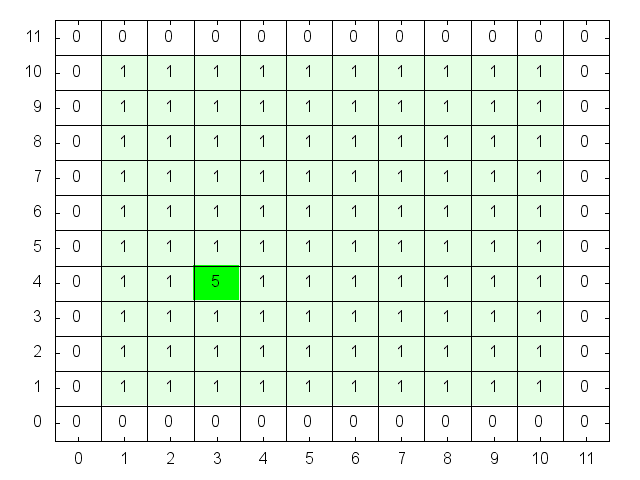
\includegraphics[width=0.7\textwidth]{plots/task_01.png}
    \caption{A simple print of an intial field.}
    \label{fig:task01}
  \end{figure}

  \begin{figure}[h!]
    \centering
      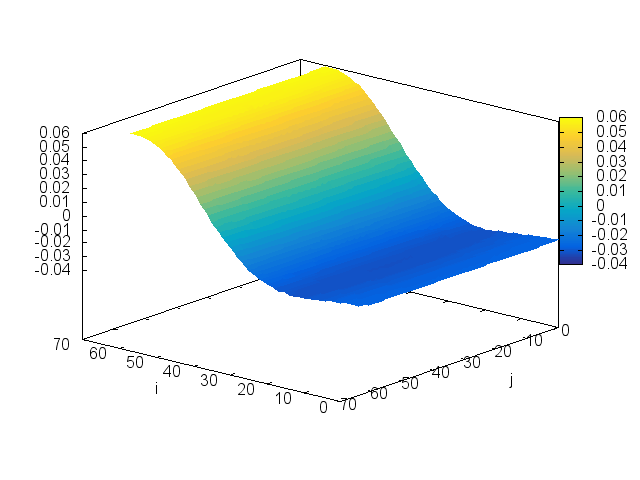
\includegraphics[width=0.7\textwidth]{plots/compute_result}
    \caption{A solution for $f(x,y) = \sin(\2\pi x)$ on a $64\times 64$ grid.}
    \label{fig:solution}
  \end{figure}

\section{Task 2}
\begin{figure}[h!]
  \centering
    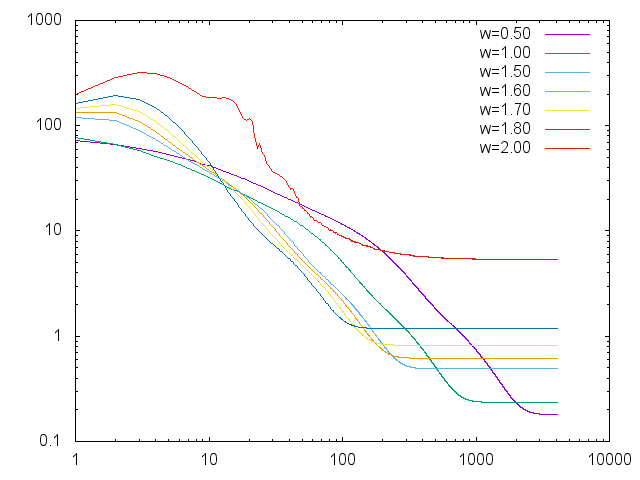
\includegraphics[width=0.7\textwidth]{plots/varying_omega.png}
  \caption{The residual as a function of the iteration count for several values of $\omega$.}
  \label{fig:varying_omega}
\end{figure}

\begin{figure}[h!]
  \centering
    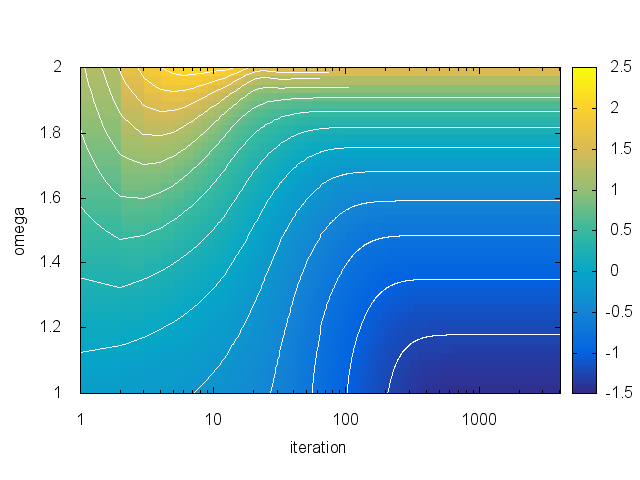
\includegraphics[width=0.7\textwidth]{plots/omega_field.png}
  \caption{The residual as a function of the iteration count for several values of $\omega$ in a contour plot.}
  \label{fig:omega_field}
\end{figure}

 Looking at figure \ref{fig:omega_field} and \ref{fig:varying_omega} we can see that surprisingly smaller values of $\omega$ perform better.
 Small values of $\omega$ correspond to reducing the effect of overshooting so that is most likely what is happening here.\footnote{or we have a bug somewhere.}
 Still, looking at figure \ref{fig:varying_omega} we can clearly see that higher values of $\omega$ (around 1.5) initial descend steeper, so the best moethod would probably be to
 use a heuristic which gradually reduces $\omega$ as the slope of the residual curve flattens out. In any case, the tolerance of $10^{-12}$ as shown in the assignment's flowchart seems to be
 rather optimistic.

\section{Task 3}
I have parallelized the solver at three points in the code. First, at the red and black loops for updating the points, and secondly when calculating the L2-norm of the residual, and third when
subtracting the mean from each point.
 The speedup as a function of the threads are plotted in figure \ref{fig:threads}.
 The results are somewhat lackluster. This could be due to the way the code is written.
  Wile most functions are inlined into the main "run" function it may still fork/join too
  often to get enough speed-up, manually inlining all the functions into a single parallel block does perform somewhat better, supporting this hypothesis. A solution might be to do multiple red-black iterations at a time
however these will still need to sync in between runs. False sharing was looked into but the static scheduler should split the work in equal sized continous chunks reducing it as much as reasonably possible.
\par We might also have been too impatient and not used a large enough grid size to see the real benefits. :)
\begin{figure}[h!]
  \centering
    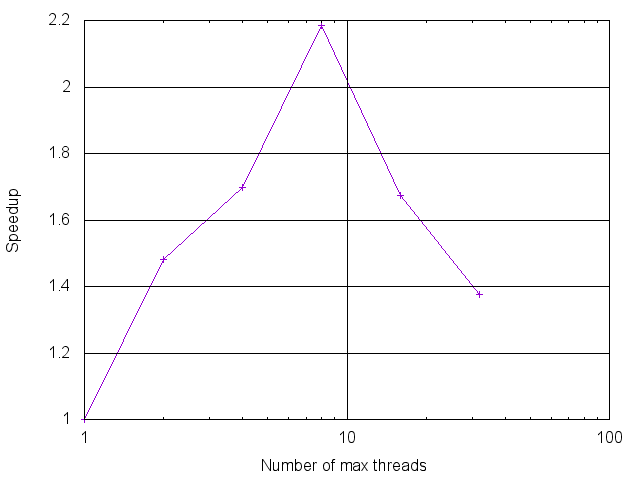
\includegraphics[width=0.7\textwidth]{plots/threading_speedup.png}
  \caption{The speedup of our algorithm for various maximum thread counts.}
  \label{fig:threads}
\end{figure}

\section{Thoughts on OpenMP}
OpenMP looks like an effective way of quickly getting a large speed-up for little work. The compiler oriented structure should also lead itself to highly optimized vendor implementations (Intel has its own runtime implementation it seems).
However, as we have noticed in Task 3 it can lead to large blocks of code if one wants to reduce the overhead of fork-joining negating some of the readability benefits over other methods of parallelizing.
The lack of more fine-grained control can also make it less efficient both in work-time and run-time I suspect if the problems become more complex (such as recursive heuristic based tasks or heavilly data-layout optimized code).
\end{document}
